\chapter{Newtonian Gravity, Gauss's Law, and the Equivalence Principle}

This chapter follows Leonard Susskind's second lecture on general relativity in the order in which the argument is actually unfolded. We begin with a brief detour about dark energy, return to Newtonian field language, reformulate gravity through Gauss's law, and then turn to Einstein's equivalence principle, light bending, and the first geometric hint of curvature. The lecture and its preserved board work are due to Leonard Susskind; the present note-making curation also owes explicit credit to LazyingArt LLC and Video2Book.

\section{Dark Energy, the Big Rip, and a Return to Newton}

The lecture opens by clearing away a lingering worry: if dark energy behaves like a repulsive component of gravity, why does it not tear atoms, planets, and galaxies apart? Susskind's answer is deliberately practical. He does not begin with cosmological field equations. He begins with a spring.

If two particles are held together by an ordinary restoring force, then to first approximation we may write
\begin{equation}
F(r)\sim -kr.
\end{equation}
A positive cosmological constant is then described, at the level of this opening heuristic, as a tiny repulsive correction proportional to distance,
\begin{equation}
F(r)\sim -kr+\lambda r.
\end{equation}
The point is not that the atom literally is a spring. The point is that for a bound system, a very small repulsive term of this type merely shifts the equilibrium position. It weakens the net restoring force slightly. It does not, under ordinary circumstances, overwhelm the binding force.

That is the basic scale argument of the opening minutes. The coefficient multiplying the repulsive term is so small that its effects become comparable to familiar binding forces only on cosmological distances. On laboratory scales it is negligible. On solar-system scales it is negligible. Even for galaxies, what it does is not to rip them apart in any immediate way, but to produce only a tiny outward correction unless one entertains much more exotic and much less credible dynamics.

\subsection{Question \& Answer}

\paragraph{Question.} Why does dark energy not tear atoms, solar systems, or galaxies apart?

\paragraph{Answer.} In the lecture's opening model, dark energy contributes a repulsive term proportional to distance, but with an extraordinarily small coefficient. In a bound system the dominant effect is therefore only a tiny shift in equilibrium. The spring gets a little weaker; it does not disappear. The ``Big Rip'' scenario would require something much more drastic, namely that the effective repulsive coefficient grows with time. Susskind treats that as bad physics, not as the ordinary consequence of a cosmological constant.

With that conceptual housekeeping out of the way, the lecture returns to the main road: we still need more Newton before we are ready for Einstein.

\section{Fields, Del, and the Gravitational Acceleration}

Susskind now slows the pace and reintroduces the notation. The operator
\begin{equation}
\nabla = (\partial_x,\partial_y,\partial_z)
\end{equation}
is not an ordinary vector with fixed magnitude and direction. It is a differential operator, but it behaves symbolically enough like a vector that the notation becomes extremely efficient.

If $\phi(x,y,z)$ is a scalar field, then its gradient is a vector field:
\begin{equation}
\nabla \phi
=
\left(
\partial_x \phi,\,
\partial_y \phi,\,
\partial_z \phi
\right).
\end{equation}
If instead $\vec v(x,y,z)$ is a vector field, then its divergence is the scalar
\begin{equation}
\nabla\cdot \vec v
=
\partial_x v_x+\partial_y v_y+\partial_z v_z.
\end{equation}
It is worth keeping the bookkeeping perfectly straight here: the gradient of a scalar is a vector, while the divergence of a vector is a scalar. The lecture momentarily stumbles verbally on this point, but the mathematical content is clear.

A scalar field is simply a scalar quantity depending on position. A vector field is a vector quantity depending on position. Gravity, in Newtonian language, is such a field.

Susskind defines the gravitational field operationally. Imagine a set of source masses $m_i$ at positions $\vec x_i$. Introduce a tiny test mass, release it at the field point $\vec x$, and observe its acceleration. That acceleration is the gravitational field:
\begin{equation}
\vec A(\vec x)=\text{acceleration of a test mass released at }\vec x.
\end{equation}

The lecture then spends a moment on sign conventions. That is not accidental. The field must point \emph{toward} the source masses, so we choose the displacement vector
\begin{equation}
\vec R_i := \vec x_i-\vec x,
\end{equation}
which points from the test mass toward the $i$th source. With that choice,
\begin{equation}
\vec A(\vec x)
=
G\sum_i m_i\frac{\vec R_i}{R_i^3}
=
G\sum_i m_i\frac{\hat R_i}{R_i^2},
\qquad
\hat R_i=\frac{\vec R_i}{R_i}.
\end{equation}
This is just Newton's inverse-square law written as a field equation at a point, with the direction carried by the vector $\vec R_i$.

\begin{figure}[ht]
\centering

\includegraphics[width=.62\textwidth]{lecture_02_figure_02.png}

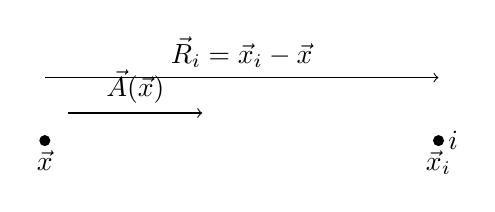
\begin{tikzpicture}[scale=1.0]
\fill (0,0) circle (2pt);
\fill (5,0) circle (2pt);
\node[below] at (0,0) {$\vec x$};
\node[below] at (5,0) {$\vec x_i$};
\node[right] at (5,0) {$i$};
\draw[->] (0.3,0.35) -- (2.0,0.35) node[midway, above] {$\vec A(\vec x)$};
\draw[->] (0,0.8) -- (5,0.8) node[midway, above] {$\vec R_i=\vec x_i-\vec x$};
\end{tikzpicture}
\caption{Field vector and source-point displacement. The board frame is preserved as documentary evidence, but the redraw fixes the convention $\vec R_i=\vec x_i-\vec x$, so that the gravitational field points toward the source without an extra minus sign.}
\end{figure}

This is the concrete Newtonian picture. But Susskind does not want to keep summing contributions one mass at a time. The next move is to summarize the whole structure in a more compact field equation.

\section{Gauss's Law and Gauss's Theorem}

To do that, we first replace discrete masses by a density field. If a small volume $\Delta V$ contains mass $\Delta m$, the mass density is
\begin{equation}
\rho=\frac{\Delta m}{\Delta V}.
\end{equation}
In the continuum limit, $\rho(\vec x)$ becomes a scalar field on space.

The Newtonian gravitational field can then be re-expressed in the local form
\begin{equation}
\nabla\cdot \vec A = -4\pi G\rho.
\end{equation}
This is Gauss's law for gravity. The minus sign matters: the field points inward toward positive mass, so what we really have physically is convergence, that is, negative divergence.

Susskind is careful here, and the notes should be equally careful. Gauss's law is a statement about nature. Gauss's theorem is different. It is a mathematical identity:
\begin{equation}
\int_V (\nabla\cdot \vec A)\,dV
=
\oint_{\partial V} A_\perp\,d\sigma.
\end{equation}
On the left we integrate the divergence over a volume. On the right we integrate the component of the field normal to the boundary. The theorem says that total divergence inside equals total outward flux across the boundary.

\begin{figure}[ht]
\centering

\includegraphics[width=.58\textwidth]{lecture_02_figure_03.png}

\begin{tikzpicture}[scale=1.0]
\draw (-2.2,-1.2) .. controls (-2.8,0.6) and (-1.2,1.7) .. (0.3,1.2)
.. controls (1.8,0.8) and (2.2,-0.2) .. (1.3,-1.3)
.. controls (0.2,-1.8) and (-1.4,-2.0) .. (-2.2,-1.2);
\draw (1.55,0.25) -- (2.15,0.25) -- (2.15,0.85) -- (1.55,0.85) -- cycle;
\draw[->] (1.85,0.55) -- (2.95,0.55);
\node[right] at (2.95,0.55) {$A_\perp$};
\node[above] at (1.85,0.85) {$d\sigma$};
\end{tikzpicture}
\caption{Surface-flux term in Gauss's theorem. The preserved board sketch makes clear that $A_\perp$ is the component perpendicular to the boundary element $d\sigma$.}
\end{figure}

At this stage the lecture is still mathematical rather than applicative. The payoff comes the moment we combine Gauss's law with Gauss's theorem and spend both on a spherically symmetric mass distribution.

\section{Spherical Symmetry and the Exterior Field}

Suppose the mass distribution is isotropic about a center. Then we surround it with an imaginary concentric sphere of radius $r$. Now the theorem and the law can be combined almost mechanically:
\begin{align}
\int_V (\nabla\cdot \vec A)\,dV
&=
\oint_{\partial V} A_\perp\,d\sigma,\\
-4\pi G\int_V \rho\,dV
&=
\oint_{\partial V} A_\perp\,d\sigma.
\end{align}
The volume integral of $\rho$ is just the enclosed mass,
\begin{equation}
\int_V \rho\,dV = M_{\mathrm{enc}}.
\end{equation}
By spherical symmetry, the normal component of the field is constant on the Gaussian sphere, so the flux side becomes
\begin{equation}
\oint_{\partial V} A_\perp\,d\sigma
=
4\pi r^2 A_r.
\end{equation}
Therefore
\begin{equation}
4\pi r^2 A_r = -4\pi G M_{\mathrm{enc}},
\end{equation}
and hence
\begin{equation}
A_r = -\frac{G M_{\mathrm{enc}}}{r^2}.
\end{equation}
If the Gaussian sphere encloses the entire body, then $M_{\mathrm{enc}}=M$, and we recover the familiar inverse-square field of Newtonian gravity.

\begin{figure}[ht]
\centering

\includegraphics[width=.62\textwidth]{lecture_02_figure_04.png}

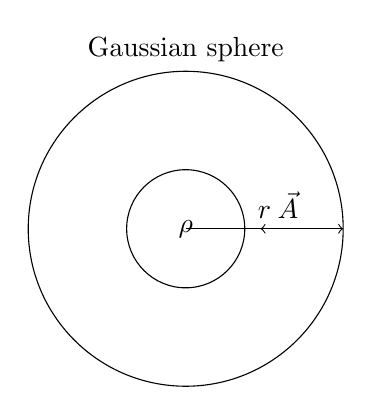
\begin{tikzpicture}[scale=1.0]
\draw (0,0) circle (2.0);
\draw (0,0) circle (0.75);
\draw[->] (0,0) -- (2.0,0) node[midway, above] {$r$};
\draw[->] (1.65,0) -- (0.95,0) node[midway, above] {$\vec A$};
\node at (0,0) {$\rho$};
\node[above] at (0,2.0) {Gaussian sphere};
\end{tikzpicture}
\caption{Gauss law with enclosed mass. The board frame documents the transition from the abstract theorem to the gravitational application; the redraw isolates the spherical symmetry used in the derivation.}
\end{figure}

This is one of the cleanest moments in the lecture. A complicated many-body sum collapses into a single statement about enclosed mass and area.

\subsection{Question \& Answer}

\paragraph{Question.} Why does only the mass inside the Gaussian sphere matter?

\paragraph{Answer.} Because Gauss's law says the flux through the sphere is determined by the integral of the density \emph{inside} the volume. Once spherical symmetry is assumed, that flux fixes the radial field on the surface. Matter outside the chosen sphere contributes zero net field there. In particular, a thin spherical shell produces no gravitational field at all in its interior, while outside the shell the field is exactly the same as if the entire mass were concentrated at the center.

This is the shell theorem in the language of flux. It is special to the inverse-square law, and Susskind rightly pauses over it.

\section{Inside the Earth: Linear Field and Harmonic Motion}

Now we repeat the same calculation, but move the Gaussian sphere \emph{inside} the Earth. The flux side still has the same form,
\begin{equation}
\oint_{\partial V} A_\perp\,d\sigma = 4\pi r^2 A_r.
\end{equation}
What changes is the enclosed mass. To make the algebra explicit, Susskind assumes a uniform density $\rho$ inside the Earth. Then the mass enclosed by the inner Gaussian sphere is
\begin{equation}
M_{\mathrm{enc}}(r)=\frac{4\pi}{3}r^3\rho.
\end{equation}
Putting this into Gauss's law gives
\begin{align}
4\pi r^2 A_r
&=
-4\pi G M_{\mathrm{enc}}(r),\\
4\pi r^2 A_r
&=
-4\pi G\left(\frac{4\pi}{3}r^3\rho\right).
\end{align}
After cancelling one factor of $4\pi$ and dividing by $r^2$, the cleaned result is
\begin{equation}
A_r = -\frac{4\pi G\rho}{3}\,r.
\end{equation}
The board discussion becomes hurried here, and the live lecture circles briefly around a missing factor of $4\pi$, but the corrected formula is the one above. It is also the one that matches the exterior formula at the Earth's surface when $M=\frac{4\pi}{3}R^3\rho$.

\begin{figure}[ht]
\centering

\includegraphics[width=.62\textwidth]{lecture_02_figure_05.png}

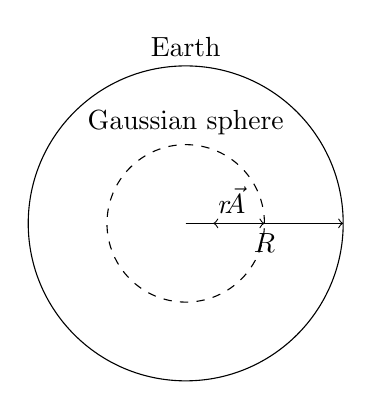
\begin{tikzpicture}[scale=1.0]
\draw (0,0) circle (2.0);
\draw[dashed] (0,0) circle (1.0);
\draw[->] (0,0) -- (1.0,0) node[midway, above] {$r$};
\draw[->] (0,0) -- (2.0,0) node[midway, below] {$R$};
\node[above] at (0,2.0) {Earth};
\node[above] at (0,1.0) {Gaussian sphere};
\draw[->] (0.9,0) -- (0.35,0) node[midway, above] {$\vec A$};
\end{tikzpicture}
\caption{Concentric spheres and enclosed-mass factor. The preserved frame gives the documentary geometry; the redraw makes explicit the inner Gaussian sphere used in the interior-field derivation.}
\end{figure}

Now the physics becomes unexpectedly elegant. Since $\vec A$ is an acceleration field, multiplying by the mass $m$ of the test particle gives
\begin{equation}
m\ddot r = -\frac{4\pi G\rho}{3}\,mr.
\end{equation}
This is exactly the equation of a harmonic oscillator. A particle displaced from the center is pulled back with a force proportional to displacement. In the idealized model of a uniform-density Earth with a frictionless tunnel drilled through it, the particle would oscillate through the Earth as though attached to a spring.

\subsection{Question \& Answer}

\paragraph{Question.} How can the field be linear in $r$ if the enclosed mass grows like $r^3$?

\paragraph{Answer.} Because Gauss's law does not equate the field directly to the enclosed mass. It equates the \emph{flux} to the enclosed mass. The flux contains the surface area factor $4\pi r^2$. Thus one power of $r$ survives:
\[
\text{field}\times r^2 \sim r^3
\qquad \Longrightarrow \qquad
\text{field}\sim r.
\]
This is exactly the point that surfaces in the classroom discussion, and it is worth preserving because it shows how the geometry of the Gaussian surface enters the physics.

The lecture briefly gestures toward gravitational potential here, but then deliberately postpones it. That is the correct place to stop. The Newtonian recap has done its work.

\section{The Equivalence Principle as a Coordinate Statement}

Susskind now pivots explicitly from old physics to new physics. The equivalence principle begins with the elevator: an observer in an accelerating cabin drops an object and sees it accelerate toward the floor exactly as though a gravitational field were present.

At first this seems almost too easy. So Susskind sharpens it mathematically. He uses the horizontal coordinate $x$ for the elevator precisely because he wants to draw an $x$--$t$ graph.

First consider uniform velocity. If the elevator moves with constant speed $v$, then the primed coordinate measured relative to the floor satisfies
\begin{equation}
x' = x-vt,
\qquad
t'=t.
\end{equation}
This is still Newtonian physics. Time is universal. If an object is at rest in the inertial frame, then $x=\text{constant}$, and differentiating gives
\begin{equation}
\dot x' = -v,
\qquad
\ddot x'=0.
\end{equation}
So a mere change to a uniformly moving frame does not create an apparent gravitational field.

Now let the elevator accelerate uniformly with acceleration $g$. Then the floor moves according to
\begin{equation}
x_{\mathrm{floor}}(t)=\frac{1}{2}gt^2,
\end{equation}
so the accelerated coordinate is
\begin{equation}
x' = x-\frac{1}{2}gt^2.
\end{equation}
If once again the dropped object is at rest in the inertial frame so that $x=\text{constant}$, then
\begin{equation}
\dot x' = -gt,
\qquad
\ddot x'=-g.
\end{equation}
This is the mathematical form of the elevator argument: inside the accelerating cabin, freely moving bodies behave exactly as though they were in a uniform gravitational field.

\begin{figure}[ht]
\centering
\begin{tikzpicture}[scale=0.9]
\draw[->] (-0.2,0) -- (4.8,0) node[right] {$x$};
\draw[->] (0,-0.2) -- (0,4.8) node[above] {$t$};
\draw (0.8,0) -- (0.8,4.2);
\draw (2.2,0) -- (3.8,4.0);
\node at (0.8,4.45) {$x=\mathrm{const}$};
\node at (3.5,4.45) {$x'=0$};
\node at (2.4,-0.45) {uniform velocity};
\end{tikzpicture}

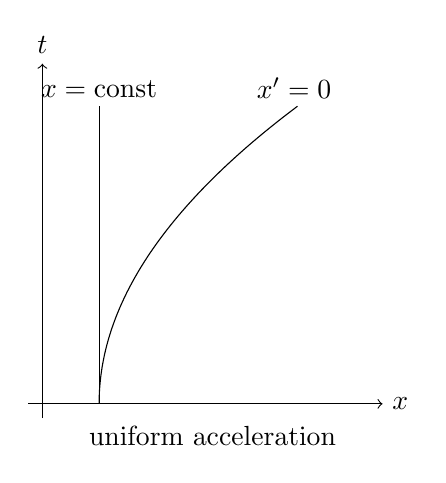
\begin{tikzpicture}[scale=0.9]
\draw[->] (-0.2,0) -- (4.8,0) node[right] {$x$};
\draw[->] (0,-0.2) -- (0,4.8) node[above] {$t$};
\draw (0.8,0) -- (0.8,4.2);
\draw plot[smooth,domain=0:2.0] ({0.8+0.7*\x*\x},{2.1*\x});
\node at (0.8,4.45) {$x=\mathrm{const}$};
\node at (3.55,4.45) {$x'=0$};
\node at (2.4,-0.45) {uniform acceleration};
\end{tikzpicture}
\caption{$x$--$t$ sketches for the moving and accelerating elevator. A uniformly accelerated floor traces a curved worldline, and the corresponding coordinate transformation produces the effective field $\ddot x'=-g$.}
\end{figure}

This is still not full relativity. Susskind says so plainly. But it already teaches the essential lesson: acceleration is encoded as a coordinate transformation, and accelerated frames correspond to curvilinear descriptions of space-time. That is the bridge to geometry.

\section{Light, Locality, and the First Hint of Curvature}

Einstein's famous move was not merely to repeat that gravity and acceleration look alike. It was to \emph{use} that statement for physics beyond Newtonian mechanics. In particular, if the laws of physics in an accelerated frame are the same as the laws of physics in a gravitational field, then the motion of light must be affected as well.

Imagine an elevator accelerating upward. A light ray is emitted horizontally from one wall. By the time it reaches the opposite wall, the elevator has risen. Therefore, as seen by the observer inside the elevator, the light ray lands lower than it would have in an unaccelerated cabin. Its path appears curved.

\begin{figure}[ht]
\centering
\begin{tikzpicture}[scale=1.0]
\draw (0,0) rectangle (6,3.5);
\draw[->] (3,3.8) -- (3,4.8) node[above] {$g$};
\fill (0.6,2.7) circle (2pt);
\draw[->] (0.6,2.7) -- (5.1,1.25);
\draw (0.6,2.7) .. controls (2.4,2.65) and (4.0,2.1) .. (5.1,1.25);
\node[left] at (0.6,2.7) {light};
\node[right] at (5.1,1.25) {hit point};
\end{tikzpicture}
\caption{Light in an upward-accelerating elevator. The apparent downward bending is the elevator version of the claim that light falls in a gravitational field.}
\end{figure}

This leads directly to Einstein's early estimate for the deflection of a ray skimming the Sun. The estimate is crude on purpose. Near closest approach, take the gravitational acceleration to be roughly its surface value,
\begin{equation}
g_\odot \approx \frac{GM}{R^2}.
\end{equation}
Approximate the time spent in the strong-field region by
\begin{equation}
\Delta t \approx \frac{2R}{c}.
\end{equation}
Then the transverse velocity acquired is
\begin{equation}
\Delta v_\perp \approx g_\odot \Delta t \approx \frac{2GM}{Rc}.
\end{equation}
For a small deflection angle,
\begin{equation}
\theta \approx \frac{\Delta v_\perp}{c}\approx \frac{2GM}{Rc^2}.
\end{equation}
This is Einstein's early estimate, before the full machinery of general relativity was in place. The lecture keeps the historical caution in view: the full relativistic result differs by a factor of two.

\subsection{Question \& Answer}

\paragraph{Question.} Can free fall completely eliminate gravity, or only locally?

\paragraph{Answer.} Only locally. For a sufficiently small elevator and over a sufficiently short time, the Earth's field can be replaced by a single accelerating frame. But the real gravitational field of the Earth is not uniform. Its direction changes from place to place, and its magnitude changes with radius. A large enough falling body feels this variation: its feet are pulled more strongly than its head, and it is squeezed sideways as neighboring free-fall lines converge. These are tidal forces. They are the obstruction to eliminating gravity globally.

That is the point at which the lecture backs away from any overstatement of the equivalence principle. Gravity is not \emph{merely} acceleration. Rather, one can trade gravity for acceleration only in a local neighborhood where tidal variations are negligible.

The last move of the lecture is to translate this local-versus-global distinction into geometry. On a flat blackboard in Cartesian coordinates,
\begin{equation}
ds^2 = dx^2+dy^2.
\end{equation}
But in more general curvilinear coordinates on the same flat surface, the distance between neighboring points takes the quadratic form
\begin{equation}
ds^2 = g_{xx}\,dx^2 + 2g_{xy}\,dx\,dy + g_{yy}\,dy^2.
\end{equation}
If the mixed term is present, the coordinate lines are not perpendicular. If the coefficients vary from place to place, the local scale and angle structure vary from place to place. Those coefficients are the metric.

Now comes the conceptual bridge that the lecture wants us to remember. Curvature is the obstruction to finding coordinates that globally flatten the geometry. Tidal forces are the obstruction to finding coordinates that globally eliminate the gravitational field. These are not two disconnected remarks. They are the opening statement of general relativity.

\section{Summary}

Lecture 2 begins with a practical detour about dark energy, but its real spine is Newtonian gravity recast as field theory. We define the gravitational field as the acceleration of a test mass, compress the many-body force law into $\nabla\cdot\vec A=-4\pi G\rho$, and then combine Gauss's law with Gauss's theorem to recover both the exterior inverse-square field and the linear interior field of a uniform-density Earth.

Only after that long Newtonian runway does the lecture make the Einstein move. An accelerated elevator produces an effective gravitational field; the corresponding coordinate transformation gives $\ddot x'=-g$; and once that idea is taken seriously for all physics, light itself must bend. But the principle is only local. Tidal forces remain, and they point beyond mechanics to geometry. The lecture ends exactly where it should: not yet with the full theory, but with the metric, curvature, and the claim that the true content of gravity lies in what cannot be transformed away.